\documentclass{UoYCSproject}
\usepackage{graphicx}
\usepackage[nottoc,numbib]{tocbibind}
\usepackage{subcaption}
\usepackage{listings}
\usepackage{wrapfig}

\usepackage[utf8]{inputenc}
\usepackage[acronym]{glossaries}

\addbibresource{Report.bib}
\title{Parallel Programming Tools for Exploring Immune System Development}
\author{Oliver Binns}
\MEng
\date{\today}
\supervisor{Dr. Fiona Polack, Dr. Kieran Alden}
\wordcount{5546}


%Approx 500 Words
\abstract{
More powerful computers are paving the way for sophisticated simulations of complex biological systems which are inaccessible to live \gls{in-vitro} study.
\acrlong{abm} has been previously used to implement this type of simulation, showing how the behaviour of a number of individual agents can contribute to the system as a whole.

The desire to create larger and more elaborate simulations, while still ensuring results can be obtained in a reasonable amount of time, makes it necessary to use parallel and distributed systems.
Creating programs and simulations that make efficient use of this parallelism can be technically challenging.
In particular it requires implementing an optimal distribution of tasks over the system and ensuring the integrity of any memory that is shared across multiple threads.
Some significant problems, including a computer science skills shortage, are slowing down the rate of progress in this area.

This project investigates the challenges and advantages of using a parallel agent-based modelling platform, \gls{FLAME GPU}, by re-implementing an existing sequential simulation of the immune-system, developed using \gls{MASON}.
During the building of the simulation, I have discovered that it is not trivial to compare between the old and new implementations, due to differences in the frameworks used.
For this reason, the final comparison will be done directly to the domain model itself.

Finally, in order to improve the mapping from the biological domain model to \gls{FLAME GPU} simulation code, I propose a \gls{mde} approach to development.
This approach reduces the parallel computing skill required to develop \gls{FLAME GPU} implementations and improves traceability from the biological domain to the implementation.
%add a little bit about the experiments you have carried out (very brief)
%and a general account of the significant findings (including any drawbacks)
}

\acknowledgements{
I would like to thank my supervisors, Fiona Polack and Kieran Alden, for their support and guidance throughout this project.
\\

I also express my thanks to Richard Paige for his pastoral support throughout this academic year, as well as his help in obtaining access to a suitable \acrshort{gpu} machine.
\\

Finally, I would also like to thank the \gls{FLAME GPU} development team at the University of Sheffield for their help in utilising the latest and pre-released features of this framework.
}

\makeglossaries
\newacronym{abm}{ABM}{Agent-Based Modelling}
\newacronym{cosmos}{CoSMoS}{Complex Systems Modelling and Simulation Infrastructure}
\newacronym{cpu}{CPU}{Central Processsing Unit}
\newacronym{cuda}{CUDA}{Compute Unified Device Architecture}
\newacronym{evl}{EVL}{Epsilon Validation Language}
\newacronym{egl}{EGL}{Epsilon Generation Language}
\newacronym{flame}{FLAME}{Flexible Large Scale Agent Modelling Environment}
\newacronym{flamegpu}{FLAME GPU}{\acrshort{flame} for the \acrshort{gpu}}
\newacronym{gpu}{GPU}{Graphics Processing Unit}
\newacronym{gpgpu}{GPGPU}{General Purpose \acrshort{gpu} programming}
\newacronym{lto}{LTo}{Lymphoid Tissue organiser cell}
\newacronym{ltin}{LTin}{Lymphoid Tissue initiator cell}
\newacronym{lti}{LTi}{Lymphoid Tissue inducer cell}
\newacronym{mason}{MASON}{Multi-Agent Simulator Of Neighborhoods}
\newacronym{mde}{MDE}{Model-Driven Engineering}
\newacronym{mimd}{MIMD}{Multiple Instruction, Multiple Data}
\newacronym{mpi}{MPI}{Message Passing Interface}
\newacronym{simd}{SIMD}{Single Instruction, Multiple Data}

%behavioural model
%complex meaning
\newglossaryentry{domain}
{
    name=Domain Model,
    description={}
}
\newglossaryentry{platform}
{
    name=Platform Model,
    description={}
}
\newglossaryentry{FLAME GPU}
{
    name=\glslink{flamegpu}{FLAME GPU},
    description={An extension of the \acrshort{flame} framework which uses \acrshort{gpu}s for parallelism}
}
\newglossaryentry{Host}
{
    name=Host,
    description={In \acrshort{gpgpu} programming, the computer containing the \acrshort{gpu} is referred to as the host}
}
\newglossaryentry{Device}
{
    name=Device,
    description={In \acrshort{gpgpu} programming, the \acrshort{gpu} hardware being used, is referred to as the device}
}
\newglossaryentry{PP}
{
    name=Peyer's Patch,
    description={Clusters of cells that form in the small intestine}
}
\newglossaryentry{LTi}
{
    name=\glslink{lti}{LTi},
    description={A moving cell that can bind to any static cell. Believed to be responsible for initiating \gls{PP} development}
}
\newglossaryentry{LTin}
{
    name=\glslink{ltin}{LTin},
    description={A moving cell that can bind to any static cell. Reponds to chemokine expression}
}
\newglossaryentry{LTo}
{
    name=\glslink{lto}{LTo},
    description={A static cell. Differentiates (divides) on stable bind with an \gls{LTin} and \gls{LTi} cell}
}
\newglossaryentry{Chemokine}
{
    name=LTo,
    description={Scientific tests conducted using computer simulation}
}
\newglossaryentry{MASON}
{
    name=\glslink{mason}{MASON},
    description={A Java framework for producing simulations using \acrshort{abm}}
}
\newglossaryentry{in-silico}
{
    name=in-silico,
    description={Scientific tests conducted using computer simulation}
}
\newglossaryentry{in-vitro}
{
    name=in-vitro,
    description={Scientific tests conducted using real biological systems under laboratory conditions}
}


\begin{document}
\pagenumbering{roman}
\maketitle
\listoffigures
\listoftables
\printglossary[type=\acronymtype]
\printglossary


%Approx 1000 words
\chapter{Introduction}
\pagenumbering{arabic}
%TELL THEM WHAT YOU WILL TELL THEM
%LIT REVIEW: TELL THEM
%RESULTS/EVAL: TELL THEM WHAT YOU TOLD THEM!
\gls{abm} has been successfully used to simulate biological systems and develop new scientific knowledge\cite{kieran_thesis, flame_keratinocyte}.
While traditional mathematical-based models are generally much more efficient to compute and produce good results when exploring how biological factors effect populations as a whole, \gls{abm} is particularly useful when considering how individuals and their interactions produce emergent system behaviour.
Mathematical-based models are limited in this aspect as they assume that each individual within the population is identical.
\gls{abm} explicitly represents each individual, meaning these can have state and attributes and are independent and fully autonomous.
%see Keratinocyte, Kieran's thesis..!
Unfortunately, these agent-based simulations require significantly more compute resources, thus taking a long time to run, particularly as simulations become more and more complex.

Here, and throughout this report, the term complexity does not necessarily refer to simulations that contains several components that are difficult to engineer.
Rather, we discuss simulations that are made up of lots of simple components that interact with each other and the environment in such a way that the system behaviour is so elaborate that it can only be predicted by running the simulation.

As these simulations often contain non-deterministic behaviour, numerous runs are required to ensure that results are statistically significant.
Consequently, it is important to ensure that the simulations make efficient use of the available compute resources, in order to gather these results in a reasonable amount of time.
The inability to obtain simulation results in a reasonable time is one of the most significant constraints upon the current use of agent-based simulations within biological research.

Another constraint affecting the adoption of \gls{abm} simulations is the ease with which they can be created.
At present, domain experts with knowledge of a particular biological system produce domain models of the system.
With the aid of software developers, these domain models are then converted into platform models.
The domain experts verify that the platform models are reasonable abstraction of the system, and they are implemented in code by the software developers.
This is the \gls{cosmos} process (Fig. \ref{fig:cosmos_process}).

\begin{figure}[htp]
\centering
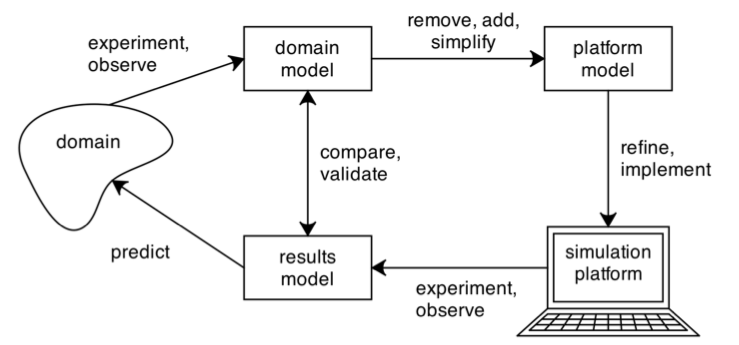
\includegraphics[width=0.75\textwidth]{Appendix/CoSMoS_Process}
\caption{\gls{cosmos} Process (Taken from \cite{mark_read_thesis})}
\label{fig:cosmos_process}
\end{figure}

A shortage of software developers who are proficient at creating efficient, parallel simulations is the current bottleneck in the adoption of the \gls{abm} simulations of processes.
If this development process can be automated by creating general solutions for common biological processes, such as cell division, it will allow simulations to be created by domain experts.
%this report discusses limitations, that are preventing this process being used to its full potential
%and explores potential solutions to this..!

%an introduction to what is to follow
%the abstract can be very specific
%Here: a bit more general (i.e. MDE and simulation concerns in general)

\section{Motivation}
%What can be gained from better modelling.. particularly biology..?
%Presentation- see justification slides!
The motivation behind this project stems from the new knowledge that could be gained from the ability to easily create efficient, parallel biological simulations.
As many biological systems cannot be fully studied \gls{in-vitro}, simulations can provide a valid alternative.
Indeed previous work has been used to produce novel biological hypotheses which have been shown to be statistically similar to those observed in the laboratory\cite[p.174]{kieran_thesis}.

%do we need citations/examples here if we are going to discuss this in more detail later on?
%is it ok to reference a later chapter?
However, these previous simulations of biological systems have had to make significant trade-offs in their implementation.
For example, 3D environments have had to be mapped into 2-dimensional simulations, cell migration into the system has been modelled as random rather than systematic\cite{kieran_thesis}, and environmental growth has been ignored\cite{phil_diss}.
%number of cell types have been reduced
The impact that these compromises have on the validity of the platform model as a representation of the domain is currently unknown.
A core motivation of this project is that, by addressing the difficulties of creating efficient, parallel, agent-based simulations, we can support simulations with fewer trade-offs in their realisation.
%can also increase the scale of the simulation

%outside of biological exploration, new understanding can..?
There are several compelling reasons for the interest in simulation of immune-related biology.
Firstly, extensive \gls{in-silico} testing could be performed much more quickly than the current \gls{in-vitro} testing, reducing the time it takes to research new drugs and cures.
Drugs and cures would be available for patients earlier, saving many lives.
Additionally, the significant financial burden of drug development, which is estimated to be around \$2.9bn\cite{drug_cost}, could be reduced, freeing up heavily contested funds for additional research. Finally, the use of animal testing could be reduced and, in the long term, eliminated completely.

\section{Project Aims}
In summary, the aims of this project are to
\begin{enumerate}
    \item Establish a firm grounding for the future development of new tools to allow fast, parallel simulations of biological systems to be easily created by non-technical users.
    \begin{enumerate}
        \item Explore the findings of the new implementation and discuss how these can be generalised to new simulations.
        \item Discuss techniques for allowing non-technical users to easily create formal models that can be transformed into new simulation implementations.
    \end{enumerate}
    \item Develop a \textbf{parallel} implementation of an existing \textbf{sequential} simulation of \gls{PP} development and explore any speed increases that can be produced by using \gls{gpgpu}.
    \item Review the use of simulations, with a particular focus on computational biology. This review explores the advantages that in-silico testing provides over \gls{in-vitro} experimentation and the problems that must be overcome for the mass adoption of biological simulations.
    
\end{enumerate}

\section{Statement of Ethics}
This project was conducted in accordance with the University of York's code of practice on ethics.
This project does not involve human participants, so guidelines on informed consent and confidentiality will be met. No confidential medical data or personal information has been used during the course of the project development. This project has involved no direct animal participation.
%[Where did the data come from?!], how was the original model created, should this be mentioned?

The ability to reduce, and ultimately replace, experimentation on animals is a positive ethical advantage of work on efficient immune-related simulation.

The simulation of the biological model is for the purpose of developing understanding of applying \gls{gpgpu} methods to an agent based model of a biological system. It will not be used its current form to publish novel biological findings and does not fully simulate a biological process.
%Software used and licences? FlameGPU is freely available / open source
%Cuda is proprietary but freely available..
%Hardware.. is this relevant?

\section{Report Structure}
This report details the work done throughout the project and 

\begin{enumerate}
    \item Chapter \ref{lit_review} gives an overview of simulations and the benefits and limitations of their use particularly with regard to computational biology.
   %\item Chapter \ref{improvements} explores some of the limitations of simulations in additional detail and proposes future solutions for these.
    \item Chapter \ref{methods} details the development of an improved, inherently parallel, implementation of PPSim (\textit{PPSim v2}) and the \gls{mde} tools that were developed to aid this work.
    \item Chapter \ref{results} evaluates the progress that this project has made towards making \textbf{fast}, parallel simulations more \textbf{accessible}.
\end{enumerate}

%Approx 3000 words for literature review
\chapter{Literature Review}
\label{lit_review}
% Aims are to:
%
% Place original work into the context of existing Literature
% Interpret major issues surrounding the topic
% Describe the relationship of each work to the others under consideration 
% Identify new ways to interpret, and shed light on any gaps in previous research
% Resolve conflicts among seemingly contradictory studies
% Determine which literature makes a significant contribution to your understanding of the topic
% Point your way to further research on your topic

\section{Simulation Background}
\label{simulation}
%Background, what are simulations used for generally
Simulations are model-based imitations of a system which feature its key characteristics and behaviours.
The system being modelled is refered to as the domain, while this simulation is known as the platform.
Computer simulations are used in a wide range of disciplines on applications such as video games, medicine, product development and even nuclear weapons.

The models of systems used in simulations may have a varying amounts of abstraction.
Simulations used for teaching will likely have models which remove significant amounts of complexity from the system.
Using abstraction to remove some of the complexity present in the domain can also help to reduce the time it takes to run the simulation, a key focus of this project.
Simulations used for video games tend to be as realistic as possible as realism has been shown to produce a higher level of immersion\cite{realism_immersion}, a highly desirable attribute of games.
%mention speculation that we live in a simulation? - simulation hypothesis, The Matrix, Elon Musk

%ABM...
In particular this project will focus on simulations created using \acrfull{abm}.
\gls{abm} is a technique that explores the autonomous behaviour and interaction between a number of individuals, known as agents.
The aim of this is to show how the individuals' behaviours interact to produce the system as a whole.
This is in contrast to more traditional mathematical top-down models which consist of a set of equations which establish relationships between a set of variables.

This chapter begins by outlining the benefits and current limitations of using simulations \textit{generally}.
It then discusses some potential solutions to some of these limitations before applying this to some of the existing simulations that have been developed using \gls{abm}.

\subsection{Benefits}
\subsubsection{Feasibility}
Exploring computer simulations is can be far more feasible than exploring a real world environment.
Video games are simulations which may allow players to experience scenarios that they may not otherwise get the opportunity to encounter.
For example, car racing games are significantly cheaper and safer than real life racing.

Real-world scientific testing may not be feasible for a number of reasons.
Simulating the aerodynamics of new car designs virtually is far quicker and cheaper than creating multiple different prototypes for physical tests.
Morality may be a factor, a good example of this is animal testing for cosmetic products or medicine.
With nuclear weapons, legality too is a key issue, as some weapon testing is banned under a number of global treaties\cite{partial_nuclear_test_ban_treaty, threshold_test_ban_treaty}.
Finally, some real-world tests may be too dangerous to perform, such as in the case of invasive medical examinations.
%SO WHAT? %POINT, EVIDENCE, EXPLANATION:
In all of these examples, computer simulation is routinely used to reduce or replace real-world testing.
%can scale be a factor? simulations can quickly model across numerous independent variables - see environmental control

\subsubsection{Reducing Complexity}
Reducing complexity through abstraction allows better understanding of the system to be gained as the complexity may initially be overwhelming.
%Removing complexity can help with understanding by removing aspects of the system that are not absolutely essential to the functionality being demonstrated.

%todo: talk about abstracting to appropriate layers..
%   clearly we only want to simulate the individuals at the level we are interested in
%   i.e. we obviously don't want to simulate our models down to the atomic/quantum level, etc.

\subsubsection{Environmental Control}
Computer simulations allow for the environment to be more easily controlled.
While the initial setup of a realistic environment may be difficult, once this has been achieved the simulations can be run in a known, constant environmental context.
It can be more easily ensured that the environment remains unaffected by any external factors.
The ability to adjust external factors and independent variables that may affect the system on demand can also be particularly useful.
This ability can be used for illustrating how different variables affect system processes.
%GIVE EXAMPLE?

%Time can be manipulated to visualise system processes at more reasonable time scales.
%A chemical process that takes a fraction of a second can be slowed down to ensure that it can be seen. 
%speed up, reverse the simulation
%easier to measure?

Furthermore, simulations allow for additional tests to be easily added at a later date.
For example, if measurements are not made for a particular variable, it can be easily added to the implementation and the simulation can be easily re-run.
This is not the case with in-vivo experimentation, which would require the laboratory to be fully set-up again, with new test-subjects for repeat experiments.

%clearly simulations may be more feasible but
%WHY are they a good alternative to real world testing?!
%accurate/realistic results produced
    %when is this the case? always? when sufficient knowledge is known?
    %relate this to laws of Physics, theoretical biology?

\subsubsection{Visualisation}
\label{visualisation}
One of the biggest benefits of simulation is the ability to graphically visualise a system or its constituent parts.
Using simulation for visualisation has number of benefits over attempting to demonstrate real world systems.
Several of these benefits translate from the previous two sections- they can be more feasible to explore than a real world environment and featuring a reduced complexity can allow the key concepts to be understood without overwhelming the user.

Simulation can be particularly useful for visualising concepts for education. 
Particularly immersive educational visualisations can also be produced using virtual and augmented reality.
The Virtuali-Tee is an educational tool that uses simulation and augmented reality to provide a view at the body's internal organs\cite{curiscope}.
Little Journey aims to reduce kids' anxiety about surgery by providing a realistic tour of their hospital ward given by animated cartoon characters\cite{little_journey}.
%use a paper to show that these are actually "immersive"

%TODO: visualisations using the CPU are VERY computationally expensive

%visualisations from the given models may not be fully accurate / may be misleading:
%   often only time-series or single-time data is available to calibrate and test the simulation..!

\subsection{Limitations and Constraints}
%ARE THERE ANY CONS?
%SHOULD simulations be used by everyone?
%Why are they not?
While simulations seem very useful across a wide number of fields, there are some significant limitations as to where and how they can be used.

\subsubsection{Insufficient Domain Knowledge}
\label{domain_knowledge}
A simulation is based on a model of a system.
A model is an abstraction from reality representing only the necessary key characteristics and behaviours of the system.
In order for the model to the be faithful to its original domain it must be able to produce demonstrably similar behaviour from similar system components.

A lack of knowledge regarding the domain of the simulation is one of the most significant constraints regarding its implementation.
If this is the case, the model produced may be incorrect or abstractions may remove necessary detail required for the system to function as expected.
Unfaithful models can also be a result of \textit{incorrect} knowledge of the domain.
For complex systems, having too many abstractions from the original domain may also invalidate the model and produce incorrect results\cite[p.8]{cosmos}.

While knowledge of a system needs to be sufficient to produce reasonable assumptions, it need not be perfect.
This is particularly the case with the type of simulation discussed later in this report.
In this case, assumptions about the domain are made %and hypotheses tested..?

\subsubsection{Compute Power}
Complex models with too few abstractions from their domain may require significant computing power to simulate. Additional abstractions may not be possible as they may invalidate the model. In these cases, cutting edge hardware may be needed for the simulation to be run in an acceptable time. 


Powerful hardware is expensive to access, so this may be a significant constraint on the ability to simulate.

%Agent-Based Modelling, which will be introduced in detail in Section \ref{abm}, models the system as a number of autonomous individuals. This technique requires significantly more compute power than the traditional top-down simulations.

%Talk about the need to speed up
%evidence behind this--!
    %machine learning paper- drive to better capture biological complexity
    %video games, better graphics and more detail
    %other examples?

%only get data on variables that have been modelled, whole system is likely not modelled, see TWA Flight 800...:
%The NTSB deemed a physical simulation appropriate as they were not convinced an available computer model would confirm the true cause of the accident.


\subsubsection{Skills Shortage}
\label{skills_shortage}
The previous section discussed reliance that complex simulations have on the latest advanced hardware capabilities.
However, advanced hardware alone will not necessarily allow a simulation to compute in a reasonable amount of time. 
%mention the concurrency- free lunch is over article findings
With modern architectures which are becoming increasingly parallel, the simulation code must be tailored to take advantage of the computing power available.
Efficient parallel programs that do this rely on the availability of experienced programmers.
May recent studies have highlighted the existance of significant computer science skills shortages, across the world\cite{digital_skills_uk, microsoft_blog}.
These skills shortages may be significantly limiting the possibility for cross-disciplinary work to utilise fast, advanced simulations.

%Computer science degrees, and related courses and apprenticeships, are proving less popular in recent years
%These are worrying trends considering the demand for digital skills by employers
    % - DIGITAL SKILLS for the UK ECONOMY, A report by ECORYS UK, JANUARY 2016

%Put simply, our nation faces an increasing shortage of individuals with the skills necessary to create and deploy the next generation of information technology.
%Despite the growing importance of computer science, it is only taught in a small percentage of U.S. schools. 
    %Microsoft Corporate Blogs, https://blogs.microsoft.com/on-the-issues/2012/12/12/investing-in-american-innovation-and-the-next-generation/

Many initiatives are being rolled out to address this issue.
Computing was added to the National Curriculum in 2013\cite{national_curriculum, teacher_training} and numerous technology companies are also creating their own campaigns\cite{apple_education, microsoft_education}.
It is likely that these will take a number of years to yield results, but should eventually mean that even domain-experts have a basic grasp of code.

\subsubsection{Bugs}
As with any form of computer program, mistakes can be made causing bugs to be present in the simulation code.
Bugs may cause the simulation to be incorrect meaning any hypotheses and results are based on incorrect data.
This is linked to, but not the same as, having insufficient domain knowledge.
Both of these limitations will cause the simulations fail silently, produce incorrect results with no immediately obvious failure[CITE].
%Failing silently is interesting: no unexpected behaviour.. this should be discussed in more detail

However, while these problems are specific to simulation, they are not dissimilar from the issues that can occur from poorly designed real-world testing.
%GIVE MORE DETAIL HERE: how can poorly designed in-vitro testing affect results in similar ways?
%As such, these limitations are no reason to dismiss simulation by themselves

%Here we are talking about refining from an initial model, which we have shown to be correct:
%This is the same concept as MDE - discussed later!
If the simulation needs to be safety-critical, developing it using formal methods and refinement may be a good way to ensure that no bugs are introduced in the code.
%CSP -> OccamPi/MASON -> Kieran is currently looking into this
%Similar to the work described later in this report: model-driven engineering!
%ensures that artifacts are inline with each other

\section{Existing Simulations}
%Previous implementations of simulations and their problems:
%In order to achieve mass-market userbase, they must be:
%EASIER TO MAKE - less technical users can work on them
%FASTER TO RUN. - more feasible, to use in experiments, more complex sims can be made

\subsection{Biological Simulations}
Computational Biology is a relatively new field of study that has been growing signficantly over the last decade[CITATION NEEDED].
Within Biology, simulation is often required as an alternative to invasive medical testing/animal testing.%NC3Rs
Simulation has even been proposed as a method for exploring a potential set of first principles and mathematics that are specific to biology which could even constitute a new subject- theoretical biology\cite{rise_article}.

\subsection{\acrlong{abm}}
\label{abm}
As previously mentioned, \gls{abm} models the autonomous behaviour of individual agents and the interaction between them.
%Write comparison of AGENTS vs OBJECTS (OOP)
Agents are often confused with objects, a commonly-used programming concept.
However, it's important to emphasize the differences between them.
In particular, while both agents and objects recognise the importance of interactions, objects are totally obediant to their method calls whereas agents have autonomy.
This means that agents can interact and react to communications according to their own agenda.

%WHY IS AGENT BASED MODELLING THE MOST RELEVANT FOR THIS PROJECT
While, \acrlong{abm} is more computationally expensive than top-down mathematical modelling, it is also more natural to model and intuitive to parallelise\cite{flame_simulation}.
Communication between individual agents can be difficult to implement in parallel but parallel communication is by no means limited to \gls{abm}.

\subsubsection{Custom Code}
While agent-based simulations can be created from scratch\cite{phil_diss} there are several distinct disadvantages to this.
Firstly, %parallalism must be ensured.
    not well tested
Finally, unlike simulations that are created using \gls{abm} libraries, they do not inherit any support for new tools and hardware that come from updates to the library.
Custom code simulations must each be updated separately with any enhancements required for.

%discuss types (and existing) simulations..

\subsubsection{Proprietary Solutions}
Some proprietary solutions for simulation creation are available.
One example of this, with a resonable level of industry support, is Biocellion\cite{biocellion}.
While it is freely-available for non-profit use, it does not help with our aim of creating a simulation platform that is simple-to-use.
It requires a level of proficiency with the Linux OS, C++ programming and familiarity with mathematical modelling concepts.
In particular, we cannot expect domain experts to be proficient at C++ programming.
%unfortunately, technical to understand- took several weeks to even install, how to cite conversation? CITE Jeff's report?

\subsubsection{\gls{MASON}}
%mason usage
%REMEMBER, this section is on EXISTING SIMULATIONS: discuss what MASON has been used for!
\gls{MASON} is a multi-agent simulation library for Java.
\gls{MASON} has been previously evaluated as the one of the fastest ABM libraries available\cite{abm_platforms_review}, however this evaluation took place over a decade ago and does not factor in any of the recent work into \acrshort{gpu} parallelism.
\gls{MASON} only supports \gls{cpu} parallelism, this will be discussed in more detail in Section \ref{cpu_v_gpu}.
%peyers patch?
%particularly well suited for these cell-based simulations as can be visualised..
%also not easy to use

\subsubsection{\gls{FLAME GPU}}
The \gls{flame} project is an attempt to make \gls{gpu}-based \gls{abm} simulations more accessible.
\gls{flame} simulations consist of two artefacts, an `XML Model File' containing the structure of agents and their channels of communication and C source code file of `Scripted Behaviour' which defines the actual behaviour of agents.
\acrfull{flamegpu} is an extension of the original version of \acrshort{flame}, where the simulations that are created are compiled down to parallelised CUDA code.
%flame is built on top of CUDA, why?
This means the simulation can take full advantage of the power of modern NVIDIA \acrshort{gpu}s.

\begin{figure}[htp]
\centering
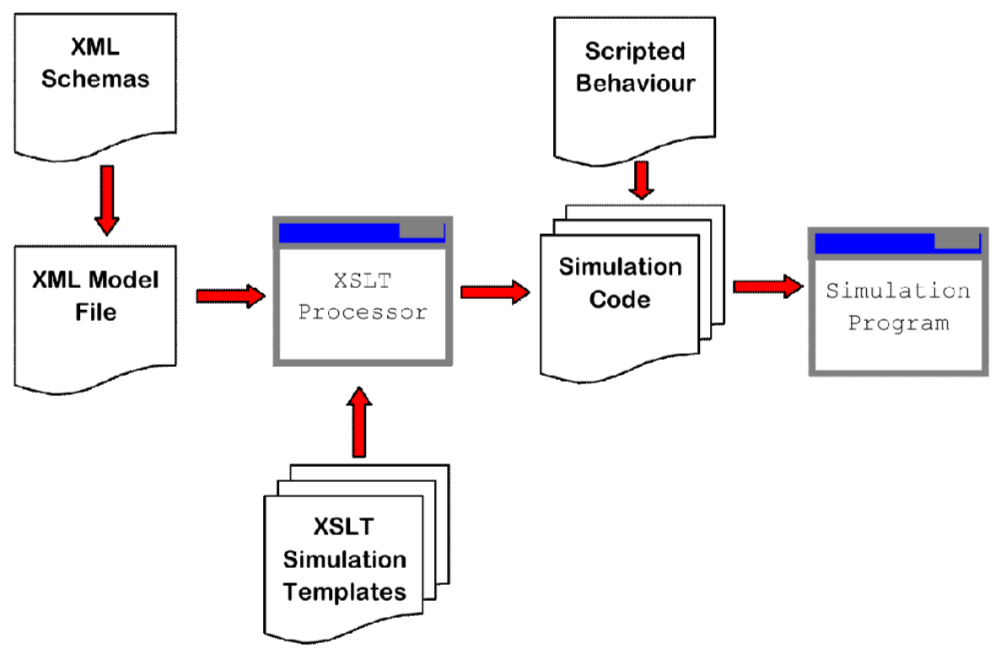
\includegraphics[width=0.6\textwidth]{Appendix/FLAME_Process}
\caption{\gls{FLAME GPU} Development Process (Taken from \cite{flame_simulation})}
\label{fig:flame_dev}
\end{figure}

\gls{flame}'s use of \gls{mde} could gives domain experts with limited programming knowledge the ability to understand and help design the simulation models, however a software engineer is still needed for the final implementation.


%partitioning is particularly effective if the vast majority of space is unpopulated
%Other specifications of FLAME GPU?

%REMEMBER, this section is on EXISTING SIMULATIONS: discuss what FLAME has been used for!

%Disadvantages
While relying on a framework such as \gls{FLAME GPU} can cause problems if support is stopped, this should be slightly less of a concern as \gls{FLAME GPU} is an open source project.
A more pressing concern with relying on any framework is that implementations are restricted by any of the framework's limitations.
For example, the current stable release of \gls{FLAME GPU} does not allow new agents to be created by the \gls{Host} between simulation steps.
%other limitations?

%Advantages
However, the \gls{FLAME GPU} framework does bring a number of advantages.
Firstly, it provides a \gls{mpi} which abstracts away from the underlying agent communication.
This \gls{mpi} supports spatial partitioning allowing messages to be passed only to nearby agents.
Communication between threads which is one of the most difficult tasks in parallel programming.
\gls{FLAME GPU} manages this communication in its entirety, meaning programmers can instead focus on ensuring the agent behaviour is correct.

%VISUALISATION COMES FREE!
\gls{FLAME GPU} also provides visualisations for simulations straight out of the box.
The benefits of visualisation are discussed in Section \ref{visualisation}.
Visualisations in \gls{FLAME GPU} run in real-time and can be useful for quickly verifying whether a simulation is behaving as expected.
%SCREENSHOT FIGURE HERE?

Many other advantages come directly from \gls{FLAME GPU}'s use of \gls{mde}.
\gls{FLAME GPU} is continuously updated to support new hardware advances, such as multicore \acrshort{gpu} architectures\cite{flame_simulation}.
\gls{FLAME GPU} simulations can always be certain of taking advantage of the latest hardware optimisations and portability features that the framework provides.
Existing simulation models that are implemented on top of \gls{FLAME GPU} may receive these performance improvements without any major code changes.
%In particular, it gives domain experts with limited programming knowledge the ability to understand and help design models.
%Additionally, the auto-generation of artifacts, such as simulation code templates, significantly lowers the boundary to entry to less advanced programmers.

Some notable benefits of \gls{mde} are not exploited in the current implementation of \gls{FLAME GPU}.
%TODO discuss these:
%migration?
%auto-generation
%auto-validation fixes?

\section{Improving Simulations}
\label{improvements}
%Section on what we need to support complex simulations
%link this to the previous chapter- discussion on current constraints on simulation:
Significant constraints on when simulations can be used were discussed in Section \ref{simulation}.
In order for simulations to become more widely adopted, some of these constraints must be overcome. 
In particular, this project focuses on two particular sections of which I believe will have the biggest immediate impact.
This section discusses the potential solutions to each of these problems.

\subsection{Ease of Creation}
A major constraint on the adoption of simulations is how difficult and time-consuming they are to create.
This constraint is exacerbated by a current shortage of experienced programmers.
Initial work to help overcome this skills shortage will likely come by providing tools that can automate work done undertaken by technical users in order to increase their productivity.

Eventually, if this technical work can be fully automated, non-technical users will be able to easily create advanced simulations.
%person-centric healthcare, custom simulations may be needed

%difficult to create a framework that allows for easy modelling of BOTH state and interaction between agents[CITE NEEDED?, no but seriously]

%As computers are getting easier to use, users are beginning to expect this even from advanced tools

\subsubsection{\acrlong{mde}}
This project has already discussed abstractions with regards to modelling for simulations.
Abstractions are also particularly useful in software engineering.
As software gets more complex, addition abstraction is generally needed in order to extract the important details of the implementation\cite[p.24]{csapp}.

\gls{mde} is a software abstraction for creating and exploiting domain models, such as those that have been previously discussed with regards to simulations.
\gls{mde} has shown a promising increase in understanding between stakeholders and can produce productivity gains when models are reused across projects\cite{mde_industry_review}.
%EPSILON, benefits of MDE?
%Domain specific modelling, etc.

\paragraph{Epsilon} Epsilon is a set of tools and languages for supporting \gls{mde}.
It provides tools for creating metamodels, model validation, model-to-model transformation, code generation and more.\cite{epsilon_book}

%Tools are a particularly important feature of mde.
%According to its website, Epsilon has a wide range of industry support.


\paragraph{Flexible Modelling}
Flexible Modelling tools could be a good method for allowing new simulations to be created more easily.
Using flexible modelling, non-technical users would be able to create sketches which can be automatically processed by tools into formal models and prototype metamodels\cite{Paige2017}.
FlexiSketch is a good example of this and provides a good tool for creating models and metamodels for software development\cite{flexisketch}.
%however.. flexible modelling is a far off goal here.?

\subsection{Speed Up}
Simulations need to be able to generate results in a realistic amount of time.
Many biological simulations include significant elements of randomness meaning must be run a large number of times in order to produce statistically significant results.
With novel applications attempting to simulate increasingly complex models, it is becoming more and more difficult to ensure that they have reasonable runtimes.
This section evaluates recent work into achieving faster simulations.
%discussed compute power above, relate this specifically to biology now!
%more complexity = more realistic = more data to process and more statistical analyses to evaluate = longer to run
%additional complexity:
    %person centric healthcare- simulations must be customisable [machine learning paper]

\subsubsection{Machine Learning}
%Talk about Kieran's original thesis and how long it took to run, and to develop the results, etc.
An upcoming paper explores the possible use of machine learning to emulate and predict the output of an existing simulator\cite{kieran_machine_learning}.
This emulation method produced some very accurate results within seconds, however it still requires an initial training set, and so does not fully remove the desire for fast simulations.
As the number of parameters increase, the training set size must also increase in order to produce accurate results.
This technique also requires expertise in machine learning which conflicts with our other aim- to make simulations more accessible.
%likely affected by Standard Machine Learning issues? Bias? Overfitting?
%harder to verify and make argument-based validation?

%2.3.2: Machine learning was on a summary of 500 executions of 500 parameter sets, not a small set of results. 
% the fact you are predicting the results of a simulator then trying to understand how that prediction relates back to the real world is another. 


\subsubsection{Parallelism}
%Trade-off, Peak Performance vs Programming Ease, this can be related to the previous section
%Complex to program, need to bear in mind:
%   Radius of the agent messages, data transfer cost is HIGH
%   Mindful of multi-thread data manipulation
Parallelism fundamentally changes the game and allows computers to keep following Moore's law even as engineers are struggling to make transisters ever smaller and smaller\cite{concurrency_revolution}.
As modern computers tend further towards parallelism to keep providing the speed-ups that have been inherent in the industry over recent years, new parallel algorithms need developing in order to take full advantage of the computing power available.

Managing parallel implementations of algorithms has significant overheads due to the need to ensure memory integrity when transfering data between parallel tasks.
The different approaches to parallelism make different trade-offs, meaning some may be more suited to a particularly task than others.
In order to ensure that the gains made by parallelising the task are not overshadowed by the overheads of managing a parallel implementation, the simulation programmer must have sufficient knowledge of the approach being used.
%Different approaches to parallelism have different tradeoffs- we need to ensure that any gains here are not overshadowed by the overheads of managing a parallel implementation- programming difficulties, data transfer costs, partitioning, reduce phase, etc;

\paragraph{Distributed Systems}
%MAPREDUCE for distributed systems could be mentioned
A distributed system is a method for running a computer program across multiple computers on a network.
Unlike parallelism that is local to a particular computer, with a distributed system there is generally no global clock to ensure that processors are kept in sync.
In order for any distributed system model to provide speed improvements, the gains provided by parallelising the data processing step must be substantial enough to overcome the time taken for data transfer between computers.

DMASON is an enhanced version of \gls{MASON} library which aims to harness unused PCs as a makeshift distributed system.
DMASON can also be set up to run on a compute cluster.

\paragraph{\acrshort{cpu} vs \acrshort{gpu}}
\label{cpu_v_gpu}
Modern computers provide two main means for parallelising code.
We are building on a previous project\cite{phil_diss} which laid the groudwork for this.
This previous project outlined the choice between \acrshort{cpu} and \acrshort{gpu} parallelism and makes the case for exploring \acrshort{gpu}s- simplisitically put, this is due to the significantly greater speed ups that can be achieved.
Indeed it has been shown that \acrshort{gpu} simulation on a standard desktop computer can easily produce performance rates that are better than those of a high-performance computing cluster\cite{flame_simulation}.
One case study even reduced the time taken for a simulation to be computed from hours on a \acrshort{cpu} to just seconds on a \acrshort{gpu}\cite{flame_keratinocyte}.
%^^ performance

\begin{figure}[htp]
\begin{subfigure}{0.50\textwidth}
\centering
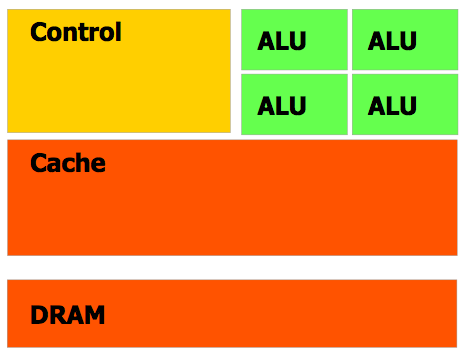
\includegraphics[width=0.8\textwidth]{Appendix/CPU}
\caption{CPU}
\label{fig:cpu_structure}
\end{subfigure}
\begin{subfigure}{0.50\textwidth}
\centering
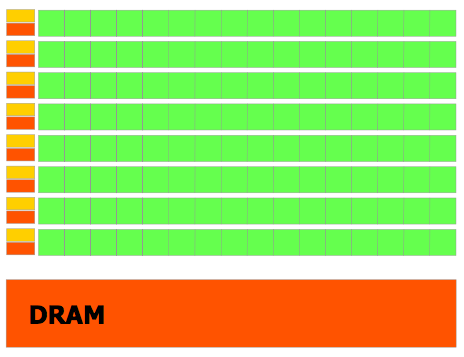
\includegraphics[width=0.8\textwidth]{Appendix/GPU}
\caption{GPU}
\label{fig:gpu_structure}
\end{subfigure}

\caption{Silicon Space Allocation (Taken from \cite[p.2]{cuda_doc})}
\label{fig:gpu_v_cpu}
\end{figure}

The key difference between \gls{cpu} and \gls{gpu} parallelism lies in the Flynn's taxonomy classification\cite{flynns_taxonomy} of architecture used by each.
\gls{cpu}s use a \gls{mimd} paradigm- this is parallelism of instruction as different \gls{cpu} cores can each be running different instructions concurrently.
Meanwhile, \gls{gpu}s use a \gls{simd} paradigm- this is parallelism of data as the same program is executed on a large quantity of data.
These differences can be most starkly visualised by observing the difference in the allocation of transistors between the two components (Fig. \ref{fig:gpu_v_cpu}). While the \gls{cpu} devotes a large amount of space to data caching and flow control, the \gls{gpu} allocates the vast majority of its capacity to data processing.\cite[p.2]{cuda_doc}

%briefly discuss jargon - device, host, etc.
%overview of the main differences:
%   parallelism of data vs parallelism of instruction
%compare speed ups that can be gained, reference Phil's project for more details

%MENTION DIFFICULTY GETTING ACCESS TO A GPU FOR TESTING:
Multiple \acrshort{cpu} cores are now commonplace in modern computers, including smartphones.
In contrast to this, dedicated \acrshort{gpu}s are normally only found in gaming PCs and consoles.
%This is changing, Apple now includes a custom \acrshort{gpu} in many of its mobile devices- metal?

\paragraph{OpenGL vs \acrshort{cuda}}
A previous project compared OpenGL and \acrshort{cuda} in detail.
%OpenGL runs on a wider number of devices, including mobile (iOS)
%frameworks, such as Apple's Metal allow significant simulations to be run, even on mobile devices

\chapter{Tools and Platform}
\section{Tools}
This project was developed on a machine running Ubuntu 16.04 with Intel i5 (650 @ 3.20 GHz) and 8GB of RAM.
The GPU utilised was an NVIDIA GeForce GTX 1050.
GPU programming utilised the latest version of CUDA (9.1).

In order to produce a working simulation of \gls{PP} formation, I have used an unreleased version (v1.5) of \gls{FLAME GPU}.
Amongst other features, \gls{FLAME GPU} v1.5 adds the ability to create agents from a host function between simulation steps.
As \gls{FLAME GPU} is developed openly, this version is freely available online\cite{flame_github}.
\gls{FLAME GPU} has been added to the project repository as a submodule, to ensure version compatibility between \gls{FLAME GPU} and \textit{PPSim v2}.

Eclipse Neon v4.6 and Epsilon v1.4 have been used with Java Runtime Environment 1.8.0 for developing the input XML model for \gls{FLAME GPU}.

Version-control for both the simulation code and this report has been managed through Git and is available on \href{https://github.com/oliver-binns/PRIY.git}{GitHub}. As this is an individual project, Git has been an acceptable solution. If the scope of the project is to expand, it may become necessary to move the modelling section of the development into a more suitable version-control system, such as EMFStore\cite{emf_store} which is specifically designed for models.

%Approx 1500 words for problem description and analysis
\section{\gls{PP} Case Study}
\label{ppsim}
This project focuses on simulation as a tool for exploring biological systems at cell level.
It uses the existing simulation of \gls{PP} development\cite{kieran_thesis} and attempts to use parallel computer architectures in order to speed this simulation up.
%proof of concept- what new knowledge has PPSim created so far?
Finally, I propose a new tool, which builds on existing work, in order to take a first step towards making efficient, parallel simulations available to non-technical users.

\subsection{The Domain Model}
The domain model for this \gls{PP} simulation is taken from an existing sequential \gls{MASON} simulation.\cite{kieran_thesis}
This model has been developed according to the \acrshort{cosmos} process.\cite{cosmos}
%Briefly detail how CoSMoS makes for better simulations

\begin{figure}[htp]
\begin{subfigure}{0.70\textwidth}
\centering
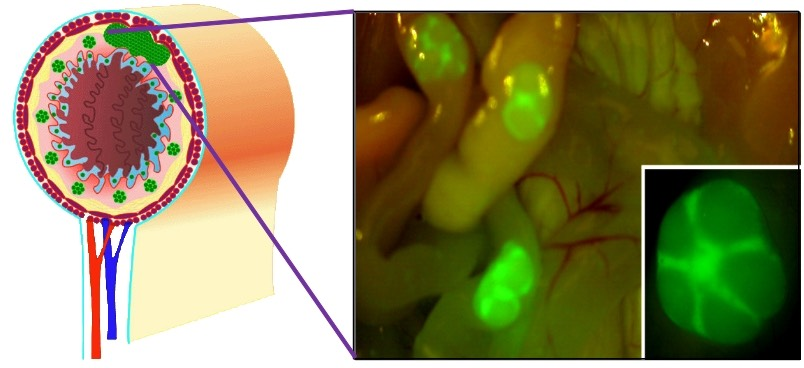
\includegraphics[width=\textwidth]{Appendix/Adult_PP}
\caption{Adult Peyer's Patch}
\label{fig:adult_pp}
\end{subfigure}
\begin{subfigure}{0.29\textwidth}
\centering
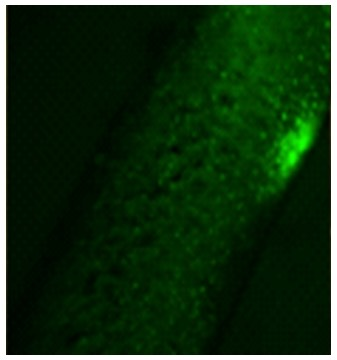
\includegraphics[width=\textwidth]{Appendix/Foetal_PP}
\caption{Foetal Peyer's Patch}
\label{fig:foetal_pp}
\end{subfigure}

\caption{(Taken from \cite{})}
\label{pp_imaging}
\end{figure}

\gls{PP}es are clusters of cells that form on the lining of the small intestine (Fig \ref{pp_imaging}).
The enviroment of the model is a 3-dimensional tube modelled in 2-dimensions.
%Environment.. 2D Plane- that wraps in the y direction?
%Agents that leave the end of the tube are n
%Agents 
In this model there are three types of agent which are all types of cells; \gls{lto}, \gls{ltin} and \gls{lti}.

Stationary \gls{lto} cells 


The model begins when \gls{lti}/\gls{ltin} cells begin migrating into the environment.
As such, at the beginning of the simulation, none of these cells are present.
\gls{lti} and \gls{ltin} cells migrate into the environment at a constant rate, such that the correct number of cells is reached at the 12 hour time-step.

Initially the \gls{lti} and \gls{ltin} cells move randomly around the environment.

\section{The Platform Model}
The simulation spans over the 72 hour period in which the \gls{PP} develops.
In this platform model there is a single \textit{active} \gls{lto} cell in the centre of the environment.
These \gls{lto} cells divide every 12 hours.
A previous project on this topic stated that \gls{lto} cell division must be performed sequentially on a host function in order to prevent new cells occupying the same space\cite{phil_diss}.
However, by adding a force resolution step, as used in previous \gls{FLAME GPU} simulations\cite{flame_keratinocyte}, this has been implemented in parallel, on the device.
As well as the speed up from parallelising the division step, implementing it feature in this way has also removed the cost of data transfer between the \gls{Device} and \gls{Host}.

There are no \gls{lto} and \gls{ltin} cells in the environment when the simulation is initialised.
A \gls{Host} function manages the migration of \gls{lto} and \gls{ltin} cells into the environment by creating these cells in random positions at a constant rate.

%Approx 2500 words for design and implementation
\chapter{Methods}
\label{methods}

%Intro Chapter:
The chapter details the simulation experiment that has been performed and the development of new tools to aid the implementation of this, and future simulations.
The experiment involved the development of a new \acrshort{gpu}-based \textit{PPSim v2} platform implementation as well as a new tool for mapping and transforming biological models into \gls{FLAME GPU} simulations.
Having previously established the current difficulties with biological simulation, this chapter also details how these are overcome in the implementation of this project.

\section{\gls{FLAME GPU}}
%HOW DOES THIS RELATE TO THE COSMOS PROCESS (ABOVE)
Building \gls{FLAME GPU} simulations requires the creation of two artifacts (Fig. \ref{fig:flame_dev}), a structural `XML Model File' which defines the agents in the system and their allowed channels for communication and a C source code file of `Scripted Behaviour' which defines the actual behaviour of agents.


A state-based platform model design is already available- the domain model for the original \gls{MASON} implementation of this simulation.
As \gls{FLAME GPU} uses state machines for each agent type in its implementation, these have been directly implemented into it.

Host cell creation into the system is a work in progress for next \gls{FLAME GPU} release?

Due to time constraints, I have not been able to implement environmental growth.
%This isn't complex to implement within FLAME GPU itself.. a step function could be used to adjust each agent's position.
%Unfortunately at present the FLAME GPU simulation sets the camera in the centre position of the environment bounds- these are determined by the INITIAL position of cells

\subsection{Epsilon}
In the creation of the \gls{FLAME GPU} XML model, I decided to implement a new tool, built using the Epsilon Modelling Framework.
The decision to use this framework was simple, as it provides all the tools required and I am already familiar with it.
The new tool contains a graphical editor which allows the \gls{FLAME GPU} `XML Model File' to be created diagramatically.
If implemented correctly, the tool should \textit{directly map} the platform model structures into the \gls{FLAME GPU} domain model.
This should significantly improve the model design experience and allow for domain experts to be kept more involved with the simulation creation.
This new process is shown as part of the \gls{cosmos} process in Fig. \ref{fig:flame_improved}.

\begin{figure}[htp]
\centering
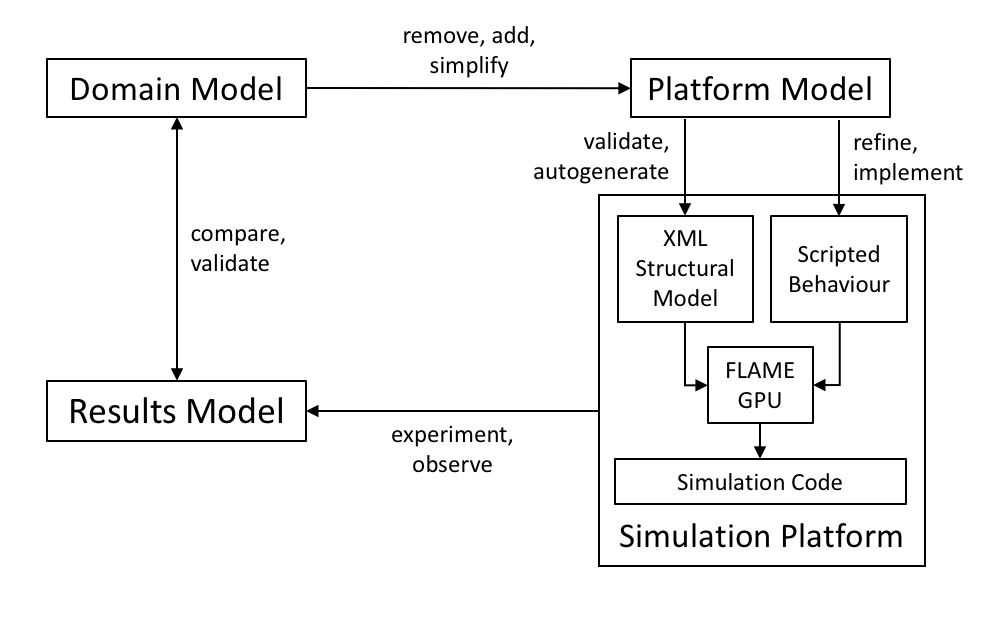
\includegraphics[width=0.7\textwidth]{Appendix/CoSMoS_FLAME}
\caption{Autogeneration of \gls{FLAME GPU} Artifact as part of the \gls{cosmos} Development Process}
\label{fig:flame_improved}
\end{figure}

Figure \ref{fig:ppsim_gmf} shows the \gls{PP} simulation created within this graphical editor. The XML model used for the final simulation was automatically generated from this diagram.

The \gls{evl} has allowed well-formedness constraints to be implemented for the \gls{FLAME GPU} input model.
This should provide intuitive feedback (Fig. \ref{fig:validation_gmf}) in cases where the model may be incorrect, in order to prevent an invalid XML model from being produced.
Quick fixes (Fig. \ref{fig:validation_quickfix_gmf}) have also been implemented to guide the user through easily correcting their invalid model.

One final benefit of this new approach to model generation, is that it makes it far simpler to .
%Hm?

%boolean transition conditions:
%critique allows users to ignore it
%BUT generally, and particularly with biological models like this:
%Transitions.. BETWEEN states require some form of external trigger?

\subsection{Testing}
As the new simulation is a re-engineering of the existing PPSim, it can inherit the validation of the existing simulation.
This requires the new simulation to be demonstrably similar with similar components, behaviours and results.
%is this the case?

Talk about how the model was tested to ensure correctness\\

%Approx 2500 words for results and evalution
\chapter{Results and Evaluation}
\label{results}


\section{Findings}
\subsection{Ease of Creation}
This proof of concept has shown that direct mappings from a biological domain model to a platform implementation are possible.
Based on this, further work is now being developed with Paul Richmond's \gls{FLAME GPU} group, to enhance the accessibility of \gls{FLAME GPU} for simulation developers.
This should allow the simulation developer to focus on getting their domain details correct, rather than battling the agent platform.
An improved mapping, which abstracts away all implementation details, could bring additional benefits in this area, including ensuring that the simulation code always supports the latest hardware features.
%Add figure, shows differences between an agent in domain model and GMF platform model-

%FLAME GPU limitations?
%future feature enhancements?

%Mention missing link in (incorrect) model from Kieran's paper 
An additional benefit of this mapping, provides traceability from the domain model through to the simulation code.
We can have greater certainty that the simulation is faithful to the domain and no bugs have been produced during the implementation.
\\\\
\textit{This work is ongoing.}

\subsection{Speed Up}


An initial aim of this project was \textit{`to explore the speed increases that can be produced by using \gls{gpgpu} programming'}.
%Model is too disimilar to Kieran's
Unfortunately the differences between the \gls{MASON} and \gls{FLAME GPU} platforms have meant that it is not trivial to compare them.
%WHY:
%Different hardware used for running? RUN on YARCC for results..?
%Mention difference between LTo cell division - force resolution step used
This initial hypothesis of the platform models being comparable is untenable.

%SPEED RESULTS..
Instead, a new hypothesis is that the platform model for the \gls{FLAME GPU} implementation is comparable to the original biological model.
If our new platform model can be shown to be similar to the original PPSim domain model, we can say that this simulation also shows Peyer's Patch development..?
%model is abstract from domain already, makes more sense to compare this to domain

%\cite{statistical_tests} could be important for evaluating the performance of \gls{FLAME GPU} against original PPSim

%Approx 1000 words
\section{Conclusion}
%NB.. INTRODUCTION + CONCLUSION MUST MATCH AND REFERENCE EACH OTHER.
%Establish a firm grounding for the future development of new tools to allow fast, parallel simulations of biological systems to be easily created by non-technical users.
%   Explore the findings of the new implementation and discuss how these can be generalised to new simulations.
%   Discuss techniques for allowing non-technical users to eas- ily create formal models that can be transformed into new simulation implementations.

%Develop a parallel implementation of an existing sequential simulation of Peyer’s Patch development and explore any speed increases that can be produced using General Purpose GPU programming (GPGPU) programming.

%Review of the use of simulations, with a particular focus on computational biology. This review should explore the advantages that in-silico testing provides over in-vitro experimentation and the problems that must be overcome for the mass adoption of biological simulations.

\section{Further Work}
\subsection{Peyer's Patch Case Study}
While the two \gls{PP} simulations are both derived from the same domain model, there are clearly significant implementation differences between these.
Future work will need to explore the meaning of the differences between simulations and whether that have any effect on their validity against the domain model.
%explore what the "differences" between the simulations "mean", specifically for PPSim and more generally

%SPARTAN?
Spartan is a tool for understanding relationships and providing novel biological insight into simulation behaviour.
Spartan was use for analysing the results of the original PPSim implementation\cite{spartan} and may provide an insight into validity of the parallel \textit{PPSim v2} implementation.

%can we produce any new hypotheses from this?

\subsection{Software Generalisibility}%IS THIS A WORD?
%Expand project for more powerful cell based simulation
%allow access to non-technical users
%flexible modelling
While the use of Epsilon has allowed for domain experts to be kept involved with the model implementation, there is still a final, most technically challenging, stage of the simulation creation where the agent behaviour is programmed.
Further work will need to study general agent behaviour in these forms of biological simulation.
The reuse of a previous simulation's implementation of cell division behaviour, has shown that at least some behaviour is common across different simulations.
The power of \gls{mde} is such that this repeated behaviour should be generalised to reduce the time needed and prevent the mistakes that occur during reimplementation of the similar software features.

On top of this, with the current implementation, technical implementation details (layer functions and agent partitioning) have become part of the model.
Ideally these should be extracted from the model implementation and automated.

\subsection{Hardware Availability}
%Talk about difficulty getting access to the necessary NVIDIA hardware
One of the greatest challenges of this project has been gaining access to NVIDIA GPU hardware.
While these are available off the shelf in most high-street computer retailers, they are not commonly found as part of standard desktop PCs, which generally containing integrated graphics hardware.
Indeed, none of the software lab PCs at the University of York contain the dedicated graphics chips required to run this software.
Future work could reevaluate whether the benefit of a cross-platform API, such as OpenGL, could outweigh the performance benefit provided by \acrshort{cuda}.
%OpenGL could be something to discuss here
%dismissed by Phil, but further exploration could be good!
%ANDY is working on this

\printbibliography
\chapter{Appendix}
\section{Simulation Parameters}

\section{Cell Data Structures}

\section{Other}

\begin{figure}[htp]
\centering
\begin{subfigure}{\textwidth}
\centering
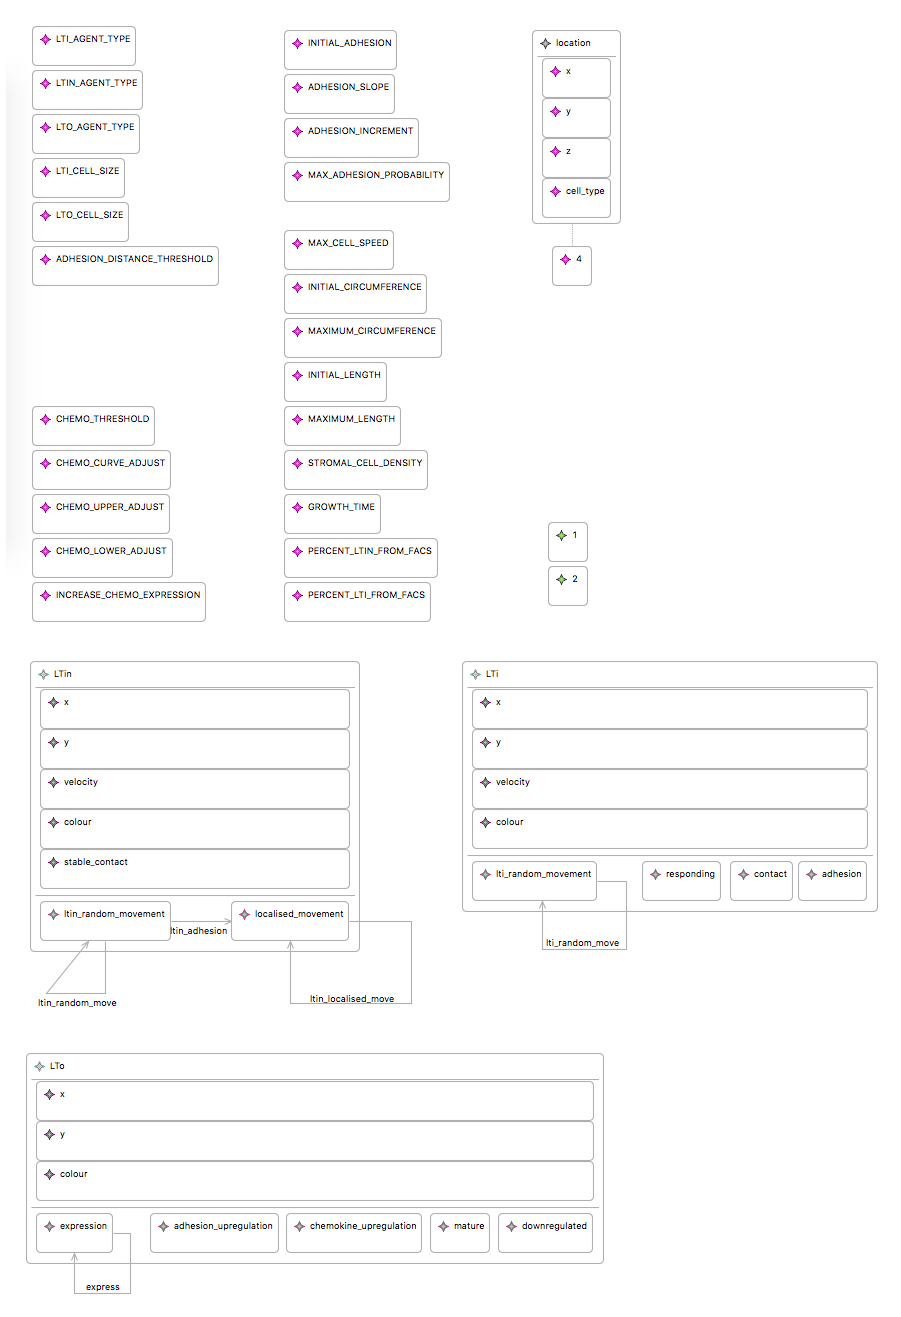
\includegraphics[width=\textwidth]{Appendix/ppsim_gmf}
\caption{Graphically produced \gls{FLAME GPU} Simulation model for Peyer's Patch}
\label{fig:ppsim_gmf}
\end{subfigure}%
\end{figure}

\begin{figure}[htp]\ContinuedFloat
\centering
\begin{subfigure}{\textwidth}
\centering
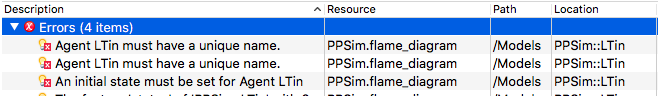
\includegraphics[width=\textwidth]{Appendix/validation_gmf}
\caption{Graphical validation using \gls{evl} constraints}
\label{fig:validation_gmf}
\end{subfigure}

\begin{subfigure}{\textwidth}
\centering
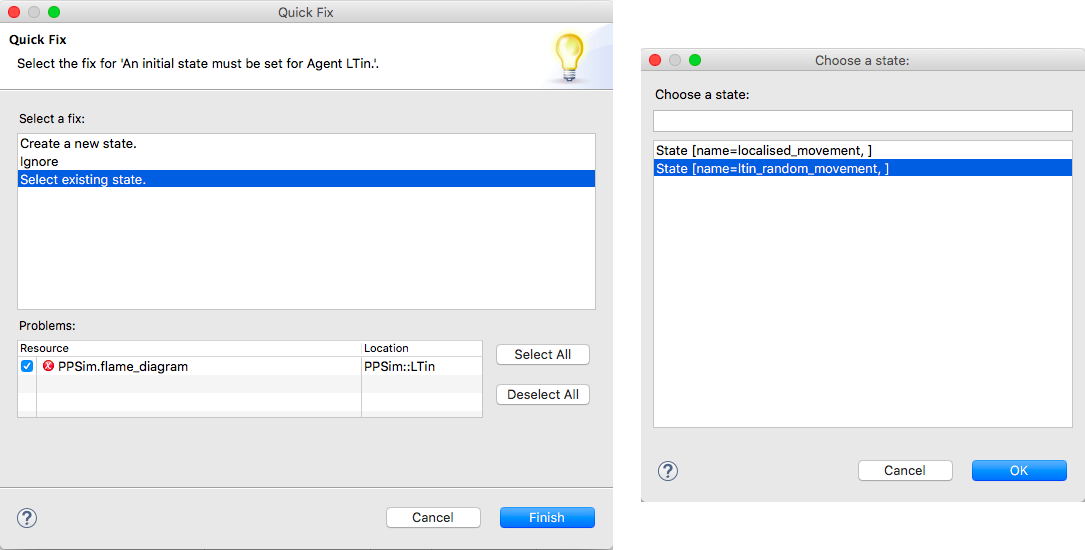
\includegraphics[width=\textwidth]{Appendix/validation_quickfix_gmf}
\caption{Quick fix of invalid model}
\label{fig:validation_quickfix_gmf}
\end{subfigure}%

\caption{Graphical Tool for creating \gls{FLAME GPU} models}
\label{fig:gmf}
\end{figure}
 
\end{document}